\documentclass[a4paper, notitlepage, 12pt]{scrartcl}
\author{Lukas Rost \\ \small{Teilnahme-ID: 48125}}
\title{Aufgabe 1 \\ \glqq Lisa rennt\grqq  - Dokumentation}
\subtitle{37. Bundeswettbewerb Informatik 2018/19 - 2. Runde \\~\\}
\date{29. April 2019}
\usepackage[ngerman]{babel}
%\usepackage[utf8]{inputenc}
\usepackage{graphicx}
\usepackage{wrapfig}
\usepackage{color}
\usepackage[dvipsnames]{xcolor}
\usepackage[hidelinks]{hyperref}
\usepackage[top=2cm, bottom=1.5cm, left=2.5cm, right=2.5cm]{geometry}
\usepackage{fancyvrb}
\usepackage{caption}
\usepackage{mathtools}
\usepackage{amssymb}
\usepackage{amsthm}
\usepackage{fancyhdr}
\usepackage{lastpage}
\usepackage{algorithm}
\usepackage{algpseudocode}

\usepackage{minted}
\fvset{breaklines=true}

\usepackage{fontspec}
\usepackage{microtype}

\usepackage{tikz}
\usepackage{svg}

\usepackage{longtable}
\usepackage{tabu}

\pagestyle{fancy}
\lhead{Lukas Rost, Teilnahme-ID: 48125}
\rhead{Aufgabe 1, Seite \thepage ~von \pageref{LastPage}}
\cfoot{ }

\newenvironment{longlisting}{\captionsetup{type=listing}}{}

\newmintedfile{python}{frame=single,linenos,samepage=false,firstnumber=1,rulecolor=\color{Gray},autogobble,breakafter={,.},fontsize=\small}

\floatname{algorithm}{Algorithmus}

\newcount\colveccount
\newcommand*\colvec[1]{
	\global\colveccount#1
	\begin{pmatrix}
		\colvecnext
	}
	\def\colvecnext#1{
		#1
		\global\advance\colveccount-1
		\ifnum\colveccount>0
		\\
		\expandafter\colvecnext
		\else
	\end{pmatrix}
	\fi
}


\begin{document}
\renewcommand{\contentsname}{\centerline{Inhaltsverzeichnis}}
 \maketitle
 \tableofcontents
 %\thispagestyle{empty}
 \setcounter{page}{1}
 
 \section{Lösungsidee}
 \subsection{Das Geometric-Shortest-Path-Problem}
 Das der Aufgabe zugrundeliegende Problem nennt sich \textit{Geometric Shortest Path} (GSP) oder auch  \textit{Euclidean Shortest Path} und stammt aus dem Bereich des \textit{Motion Planning}. Bei diesem Problem ist ein punktförmiger Roboter (oder auch eine Schülerin namens Lisa) gegeben, der/die sich an einer Startposition $p_{start}$ in einem kartesischen Koordinatensystem befindet. In diesem Koordinatensystem befinden sich mehrere als Polygone modellierte Hindernisse, wobei jedes einzelne Polygon durch seine Eckpunkte gegeben ist.\footnote{In dieser Dokumentation wird angenommen, dass die Punkte entgegen dem Uhrzeigersinn sortiert sind, sonst muss dies vorher geschehen.} Weiterhin ist eine Position $p_{ziel}$ gegeben. Nun soll ein möglichst kurzer Weg von $p_{start}$ zu $p_{ziel}$ gefunden werden, wobei dieser nicht durch Hindernisse führen soll.\footnote{Zumindest nicht, wenn Lisa als Zielposition nicht das Krankenhaus erreichen will.}\cite{Src:noem} \\ \\
 Das hier gegebene Problem unterscheidet sich von GSP dadurch, dass keine Position $p_{ziel}$, sondern ein Strahl $s_{ziel}$ (in Form eines beliebigen Punktes auf dem Strahl) erreicht werden soll. In diesem Fall handelt es sich dabei um die y-Achse ($x=0$ mit $y \geq 0$). Zusätzlich soll nicht unbedingt der Weg optimiert werden, sondern die Startzeit, die abhängig von der Länge des Weges und der für jeden Punkt des Strahls unterschiedlichen Zielzeit ist. Diese Zielzeit kann mithilfe des Abstands des Punktes vom Ursprung berechnet werden. \\ \\
 Das Geometric-Shortest-Path-Problem wird im Allgemeinen in zwei Schritten gelöst: Zunächst wird ein Sichtbarkeitsgraph erstellt, auf welchem dann Dijkstras Algorithmus ausgeführt wird.\footnote{Es existieren natürlich auch andere Herangehensweisen wie eine Grid- oder Intervall-basierte Suche, die das Problem jedoch nicht exakt lösen können und deshalb hier nicht geeignet sind.} Zur Lösung des hier gegebenen Problems wird jedoch ein zusätzlicher Schritt benötigt, der auf der Lösung des Problems ohne Hindernisse basiert. Diese drei Algorithmen sollen in den folgenden Abschnitten vorgestellt und näher erläutert werden.
 \begin{figure}[H]
 	\centering 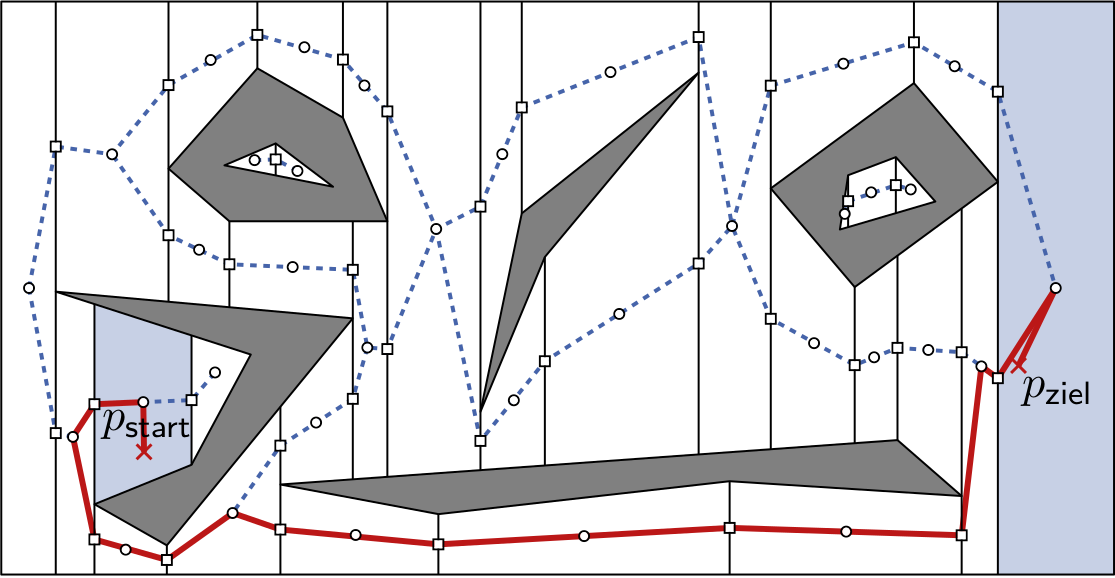
\includegraphics[scale=0.35]{pics/gsp}
 	\caption{Illustration des GSP-Problems (aus \cite{Src:noem})}
 \end{figure}
 \subsection{Erzeugung eines Sichtbarkeitsgraphen}
 Es lässt sich beobachten, dass der kürzeste $s$-$t$-Weg (dabei sei $s$ die Startposition und $t$ die Zielposition) in einem solchen Koordinatensystem ein Polygonzug sein muss, dessen innere Knoten Knoten (bzw. Ecken) der Hindernisse sind. Andernfalls wäre es immer möglich, einen kürzeren Weg zu konstruieren, der über einen Hindernisknoten führt.\cite{Src:noem} Ausgehend davon lässt sich ein sogenannter Sichtbarkeitsgraph erzeugen, bei dem es sich um einen gewichteten, ungerichteten Graphen handelt. \\ \\
 Für eine Polygonmenge $S$ mit Knotenmenge $V(S)$ sei dieser definiert als $G_{vis}(S) = (V(S),E_{vis}(S))$. Dabei ist $E_{vis}(S)$ die Menge der Knotenpaare von $S$, sodass die dazwischenliegende Strecke kein Polygon (bzw. das Innere eines Polygons) schneidet. Mathematisch ausgedrückt bedeutet das $E_{vis}(S) = \{ uv | u,v \in V(S)$ und $\overline{uv} \subset C_{free} = \mathbb{R}^{2} \setminus \bigcup S \}$. Das Gewicht einer Kante sei dabei als euklidischer Abstand der beiden Endpunkte definiert. \\ \\
 Wenn man $S^{*}$ als $S \cup \{s\}$ definiert (bei normalen Sichtbarkeitsgraphen wird auch $t$ hinzugefügt) und den Sichtbarkeitsgraphen dafür analog, kann man damit das GSP-Problem lösen. Nun entspricht der kürzeste $s$-$t$-Weg, der Hindernisse vermeidet, einem kürzesten Weg in $G_{vis}(S^{*})$.
 \subsubsection{Naiver Ansatz}
 $G_{vis}(S^{*})$ lässt sich nun naiv in $\mathcal{O}(n^3)$ berechnen, wobei $n = |V(S^*)|$. Dazu bestimmt man für jeden Knoten $u \in V(S*)$ die von ihm sichtbaren Knoten $v$. Dabei muss man für jede Strecke $\overline{uv}$ prüfen, ob sie eine der $|E_{vis}(S^*)| = \mathcal{O}(n)$ in Frage kommenden Hinderniskanten schneidet. Die Bestimmung der von $u$ sichtbaren Knoten ist somit in $\mathcal{O}(n^2)$ durchführbar und insgesamt ergibt sich eine Laufzeit von $O(n^3)$. \\ \\
 Die Funktionsweise des naiven Algorithmus wird auch in folgendem Pseudocode deutlich: 
 \begin{algorithm}[H]
 \begin{algorithmic}
 	\Function{visibilityGraph}{$S$}
 	\State $G = (V(S),E) \gets$ leerer Sichtbarkeitsgraph
 	\ForAll{Knoten $v \in V(S)$}
 	\Comment{\small{$\mathcal{O}(n)$}}
 	\ForAll{Knoten $w \in V(S) \setminus \{ v \}$}
 	\Comment{\small{$\mathcal{O}(n)$}}
 	\ForAll{Kante $e \in E_{vis}(S)$}
 	\Comment{\small{$\mathcal{O}(n)$}}
 	\If{$\overline{vw}$ schneidet keine der Kanten $e$}
 	\State $E \gets E \cup \{vw\}$
 	\EndIf
 	\EndFor
 	\EndFor
 	\EndFor
 	\State \Return $G$
 	\EndFunction
 \end{algorithmic}
\caption{Naiver Algorithmus}
\end{algorithm}
\newpage
 \subsubsection{Der Lee-Algorithmus}
 Es ist jedoch auch möglich, die Bestimmung der von $u$ sichtbaren Knoten in $\mathcal{O}(n \cdot \log n)$ durchzuführen, wodurch sich insgesamt eine Laufzeit von $\mathcal{O}(n^2 \cdot \log n)$ ergibt. Der dazu notwendige Algorithmus ist der Algorithmus von D. T. Lee. Durch dessen geringere Laufzeit lässt sich insbesondere bei großen Eingaben eine deutliche Verbesserung erreichen. \\ \\
 Es existieren zwar noch schnellere Algorithmen wie der nach Overmars und Welzl in $\mathcal{O}(n^2)$ oder der nach Ghosh und Mount in $\mathcal{O}(n \cdot \log n + E)$\cite{Src:kitz}. Doch die damit erreichten Verbesserungen sind nur in speziellen Fällen wirklich bemerkbar, während die Implementierung deutlich schwieriger ist. \\ \\
 Lees Algorithmus ist grundlegend ähnlich aufgebaut, muss jedoch für jede Strecke $\overline{uv}$ nur noch eine Hinderniskante prüfen, welche in $\mathcal{O}(\log n)$ bestimmt werden kann. Dies wird auch in folgendem Pseudocode deutlich:
 \begin{algorithm}[H]
 \begin{algorithmic}
 	\Function{visibilityGraph}{$S$}
 	\State $G = (V(S),E) \gets$ leerer Sichtbarkeitsgraph
 	\ForAll{Knoten $v \in V(S)$}
 	\Comment{\small{$\mathcal{O}(n)$}}
 	\State $W \gets$ \Call{visible\_vertices}{v,S}
 	\Comment{\small{$\mathcal{O}(n \cdot log~n)$}}
 	\State $E \gets E~ \cup \{vw~|~w \in W \}$
 	\EndFor
 	\EndFunction
 \end{algorithmic}
 \caption{Der Algorithmus von Lee}
 \end{algorithm}
 Der Algorithmus in der Methode \texttt{visible\_vertices} benutzt dabei eine sogenannte rotierende \emph{Sweep line} beziehungsweise \emph{Scan line}. Diese Sweep line fegt (\glqq sweept\grqq) den zweidimensionalen Raum aus, wobei sie durch den gesamten Raum bewegt wird, bis alle Objekte (in diesem Fall die Knoten) besucht und verarbeitet wurden. Im Falle von Lees Algorithmus rotiert die Sweep line (mathematisch gesehen ein Strahl) um dem Startpunkt $v$ gegen den Uhrzeigersinn. \\ \\
 Am Anfang zeigt die Sweep line nach rechts (parallel zur x-Achse) und rotiert so lange gegen den Uhrzeigersinn, bis sie einen Punkt trifft, der auf Sichtbarkeit überprüft werden muss. Dazu wird eine Liste der offenen Kanten geführt, mit denen sich die Sweep line aktuell überhaupt schneiden kann und die damit relevant sind.\cite{Src:pyvistwo} Anfangs werden dabei einmal alle Kanten daraufhin überprüft, ob sie sich mit der Sweep line (in der Anfangsstellung) schneiden. Entsprechend wird dann diese Liste initialisiert. \\ \\
 Trifft die Sweep line auf einen Punkt $a$, werden deshalb alle Kanten überprüft, deren Endpunkt $a$ ist. Liegt eine Kante bezüglich der Sweep line im Uhrzeigersinn (\emph{clockwise side}), kann sie, sofern sie enthalten ist, aus der Liste der offenen Kanten entfernt werden, da die Sweep line bei Bewegung gegen den Uhrzeigersinn nie wieder mit ihr in Berührung kommt. Liegt die Kante dagegen entgegen des Uhrzeigersinns (\emph{counter-clockwise side}), so muss sie zu den offenen Kanten hinzugefügt werden, da sich die Sweep line im Folgenden mit ihr schneiden kann. \\ \\
 So werden in diesem Beispiel (siehe nächste Seite) am Punkt $a$ die Kanten $\overline{ab}$ und $\overline{ac}$ hinzugefügt, da sie bezüglich der Sweep line gegen den Uhrzeigersinn (auf ihrer linken Seite) liegen. In Punkt $b$ kann $\overline{ab}$ dagegen wieder entfernt werden, da sie rechts der Sweep line liegt. Hier wird dann jedoch $\overline{bc}$ hinzugefügt.
  \begin{figure}[H]
 	\centering 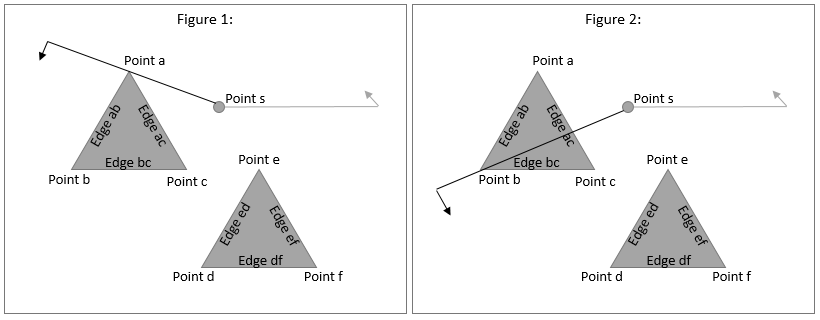
\includegraphics[scale=0.6]{pics/lee_figure1}
 	\caption{Illustration des Konzepts der \emph{Sweep line} (aus \cite{Src:pyvistwo})}
 \end{figure}
Es lässt sich zeigen, dass sogar nur diejenige offene Kante geprüft werden muss, welche am nächsten an $v$ liegt, d.h. diejenige, für die der Schnittpunkt mit der Sweep line am nächsten an $v$ liegt. Um diese Kante schnell zu bestimmen, muss man die Kanten nach der Distanz zum Schnittpunkt ordnen. Dies lässt sich zum Beispiel mit einem balancierten binären Suchbaum wie einem \emph{AVL-Baum} erreichen.\footnote{Die Funktionsweise eines AVL-Baums sei hier als bekannt vorausgesetzt.}\cite{Src:pyvistwo} Die \texttt{visible\_vertices}-Funktion sieht nun also bei einer Formulierung als Pseudocode ungefähr so aus:
\begin{algorithm}[H]
\begin{algorithmic}
	\Function{visible\_vertices}{$v,S$}
	\State $w \gets sort(V(S) \setminus \{v\} )$
	\Comment{Sortieren der Knoten (siehe unten)}
	\State $s \gets v + \lambda \cdot \colvec{2}{1}{0}$ mit $\lambda \in \mathbb{R}^+$
	\Comment{Sweep line initialisieren}
	\State{$T \gets binarySearchTree()$}
	\State{$W \gets \emptyset$}
	\ForAll{Kante $e \in E(S)$}
	\If{$e \cap s \neq \emptyset$}
	\Comment{alle Kanten, die die Sweep line schneiden}
	\State{$T \gets T \cup e$}
	\EndIf
	\EndFor
	\ForAll{Knoten $w_i \in w$}
	\Comment{in sortierter Reihenfolge}
	\State{Rotiere $s$ so, dass er $w_i$ schneidet}
	\ForAll{Kante $e$ mit Endpunkt $w_i$}
	\If{$e$ rechts von $s$}
	\State{$T \gets T \setminus \{e\}$}
	\Comment{Kante entfernen}
	\EndIf
	\EndFor
	\If{\Call{visible}{$w_i$}}
	\Comment{ist sichtbar}
	\State{$W \gets W \cup w_i$}
	\EndIf
	\ForAll{Kante $e$ mit Endpunkt $w_i$}
	\If{$e$ links von $s$}
	\State{$T \gets T \cup \{e\}$}
	\Comment{Kante hinzufügen}
	\EndIf
	\EndFor
	\EndFor
	\State{\Return $W$}
	\EndFunction
\end{algorithmic}
\caption{Bestimmung der sichtbaren Knoten bzw. Punkte im Lee-Algorithmus}
\end{algorithm}
Das Sortieren der Knoten erfolgt dabei anhand ihrer Polarkoordinaten relativ zu $v$. Dabei wird zuerst nach kleinerem Winkel zu $s$ und dann, falls dieser gleich sein sollte nach kleinerem Abstand zu $v$ sortiert. Die Formulierung \emph{links} im Pseudocode bedeutet entgegengesetzt dem Uhrzeigersinn und \emph{rechts} bedeutet im Uhrzeigersinn. \\
\begin{algorithm}[H]
\begin{algorithmic}
	\Function{visible}{$w_i$}
	\If{$\overline{vw_i}$ schneidet das Innere des Polygons, dessen Knoten $w_i$ ist}
	\State \Return false
	\EndIf
	\If{$w_{i-1}$ nicht auf der Geraden durch $\overline{vw_i}$}
	\If{$\overline{vw_i} \cap smallest(T) = \emptyset$}
	\State \Return true
	\Else
	\State \Return false
	\EndIf
	\ElsIf{$not$ \Call{visible}{$w_{i-1}$}}
	\State \Return false
	\Else
	\State{Überprüfe alle Kanten in $T$ auf Schnitt mit $\overline{vw_i}$ und ...}
	\State \Return false
	\State{.. falls Schnitt mit einer der Kanten}
	\EndIf
	\State \Return true
	\EndFunction
\end{algorithmic}
\caption{Sichtbarkeitsprüfung im Lee-Algorithmus}
\end{algorithm}
\hspace*{-1em}Diese Funktion \texttt{visible} prüft dabei ganz einfach die Sichtbarkeit eines Knotens. $smallest(T)$ gibt die kleinste Kante im Suchbaum an, sofern diese existiert.
 \subsection{Der Dijkstra-Algorithmus}
 Um nun im Sichtbarkeitsgraphen einen kürzesten Pfad vom Startknoten $s$ zu allen anderen Knoten zu bestimmen, was für die Lösung des Problems notwendig ist, kann man Dijkstras Algorithmus verwenden. Dieser arbeitet nach dem Greedy-Prinzip, bei dem in jedem Schritt ein optimaler Folgezustand gewählt wird, der das aktuell beste Ergebnis verspricht. Er arbeitet grundlegend wie folgt:
 \begin{enumerate}
 	\item Weise allen Knoten die beiden Eigenschaften „Distanz“ und „Vorgänger“ zu. Initialisiere die Distanz im Startknoten $s$ mit 0 und in allen anderen Knoten mit $\infty$.
 	\item Solange es noch unbesuchte Knoten gibt, wähle darunter denjenigen mit minimaler Distanz aus und
 	\begin{enumerate}
 		\item speichere, dass dieser Knoten schon besucht wurde.
 		\item Berechne für alle noch unbesuchten Nachbarknoten die Summe des jeweiligen Kantengewichtes und der Distanz im aktuellen Knoten.
 		\item Ist dieser Wert für einen Knoten kleiner als die dort gespeicherte Distanz, aktualisiere sie und setze den aktuellen Knoten als Vorgänger.
 	\end{enumerate}
 \end{enumerate}
Der Dijkstra-Algorithmus hat eine Laufzeit von $\mathcal{O}((|V|+|E|) \cdot \log |V|)$ (bei Implementierung mit einer Vorrangwarteschlange). Da der Algorithmus den entsprechenden Weg durch das Setzen eines Vorgängers ebenfalls bestimmt, kann auch dieser selbst ausgegeben werden.
 \subsection{Lösung des Problems ohne Hindernisse}
 Damit man nun diese spezielle Abwandlung des Problems lösen kann, sollte man zunächst einmal versuchen, das Problem ohne Hindernisse zu lösen, wie dies die Aufgabenstellung auch \emph{sehr} unauffällig nahelegt. \\ \\
 Zunächst lässt sich feststellen, dass es ausschließlich sinnvoll ist, Punkte mit einer y-Koordinate $\geq$ der y-Koordinate von Lisas Haus als Zielpunkte zu wählen. Sonst würde der Abstand zwischen Start- und Zielpunkt größer, während die Abfahrtszeit des Busses früher läge, was insgesamt für Lisa ein früheres Aufstehen bedeuten würde. \\
\begin{wrapfigure}{r}{0.25\textwidth}
	\begin{tikzpicture}
		\coordinate[label=left:$A$] (A) at (0,1);
		\coordinate[label=right:$P$] (P) at (3,1);
		\coordinate[label=left:$C$] (C) at (0,2);
		\draw (A) -- node[below] {$x$} (P);
		\draw (P) -- node[above] {$l$} (C);
		\fill (A) circle (2pt);
		\fill (P) circle (2pt);
		\fill (C) circle (2pt);
		\draw [<->,thick] (0,1.5) node[left] {$b$} (0,3) node (yaxis) [above] {$y$}
		|- (3.5,0) node (xaxis) [right] {$x$};
	\end{tikzpicture}
\end{wrapfigure}
 Betrachten wir nun die nebenstehende Situation, in der $P(x_p|y_p)$ Lisas Haus darstellt und $C(x_c|y_c)$ den optimalen Zielpunkt mit $y_c \geq y_p$. Die Zeit, die der Bus für die Strecke $b$ benötigt, berechnet sich mit $v_b$ als Geschwindigkeit des Busses zu
 \begin{equation}
 t_B = \frac{b}{v_B}
 \end{equation}
 Die Zeit, welche Lisa für die Strecke $l$ benötigt, berechnet sich äquivalent zu
 \begin{equation}
 t_L = \frac{l}{v_L} = \frac{\sqrt{x^2 + b^2}}{v_L}
 \end{equation}
 da das Dreieck rechtwinklig ist. Um nun den optimalen Punkt $C$ zu finden, ist es nötig, den Term $t_L - t_B$ abhängig von der Strecke $b$ zu minimieren. Dies lässt sich einfach mit dem aus der Kurvendiskussion bekannten Ansatz über die erste Ableitung erreichen. Dann ergibt sich:
 \begin{equation}
 \begin{split}
 \frac{d (t_L - t_B)}{db} & =  \frac{d}{db} (\frac{\sqrt{x^2 + b^2}}{v_L} - \frac{b}{v_B}) \\
 & = \frac{1}{v_L} \cdot \frac{2 \cdot b}{2 \cdot \sqrt{x^2 + b^2}} - \frac{1}{v_B} \\
 & = \frac{1}{v_L} \cdot \frac{b}{\sqrt{x^2 + b^2}} - \frac{1}{v_B}
 \end{split}
 \end{equation}
 Setzt man diese Ableitung nun gleich $0$, erhält man:
 \begin{align}
 \frac{1}{v_L} \cdot \frac{b}{\sqrt{x^2 + b^2}} - \frac{1}{v_B} &= 0 \\
 \frac{1}{v_L} \cdot \frac{b}{\sqrt{x^2 + b^2}} &= \frac{1}{v_B} \\
 b &= \frac{v_L}{v_B} \cdot \sqrt{x^2 + b^2} \\
 b^2 &= \frac{v_L^2}{v_B^2} \cdot (x^2 + b^2) \\
 (1 - \frac{v_L^2}{v_B^2}) \cdot b^2 &= \frac{v_L^2}{v_B^2} \cdot x^2 \\
 b^2 &= \frac{v_L^2}{v_B^2} \cdot \frac{1}{(1 - \frac{v_L^2}{v_B^2})} \cdot x^2 \\
 b &= \frac{v_L}{v_B} \cdot \frac{1}{\sqrt{1 - \frac{v_L^2}{v_B^2}}} \cdot x
 \end{align}
 Für den optimalen Zielpunkt $C$ gilt somit $x_c = 0$ und $y_c = y_p + \frac{v_L}{v_B} \cdot \frac{1}{\sqrt{1 - \frac{v_L^2}{v_B^2}}} \cdot x_p$. \footnote{Ich habe keine Ahnung, warum das wie der Lorentzfaktor aus der Relativitätstheorie aussieht.} Setzt man die in der Aufgabenstellung gegebenen Geschwindigkeiten ein. ergibt sich: $y_c = y_p + \frac{\sqrt{3}}{3} \cdot x_p$
 \subsection{Kombination der Ansätze}
 Um das Problem nun lösen zu können, muss man beide Ansätze (mit und ohne Hindernisse) kombinieren. Dazu bestimmt man zu jedem Knoten/Punkt $p$ in der Eingabe einen (von mir so bezeichneten) \textit{Companion}-Punkt $c$, indem man die im vorigen Abschnitt berechnete Gleichung auf diesen Punkt anwendet. Dieser Punkt $c$ ist dann der optimale Punkt, um von $p$ aus die y-Achse zu erreichen und dabei möglichst spät starten zu müssen. \\ \\
 Da es jedoch sein kann, dass $c$ von $p$ nicht sichtbar ist (ein Hindernis liegt dazwischen), muss man eine Sichtbarkeitsprüfung durchführen. Dazu betrachtet man $c$ einfach bei der Erstellung des Sichtbarkeitsgraphen, genauer bei der Ermittlung der sichtbaren Punkte von $p$ aus (und nur dabei, denn für alle anderen Punkte hat $c$ keine Relevanz). \\ \\
 Nun kann man mithilfe des Dijkstra-Algorithmus' die kürzesten Wege zu allen Companion-Knoten berechnen. Aus diesen und der Lage der Companion-Punkte (aus dieser bestimmt sich die Zeit, an der der Bus dort vorbeifährt) lässt sich dann für jeden Companion-Punkt die spätestmögliche Startzeit am Startpunkt $s$ bestimmen, wenn man an diesem Companion-Punkt auf den Bus treffen will. \\ \\
 Der Companion-Punkt mit der spätesten spätestmöglichen Startzeit ist der Punkt, an dem Lisa auf den Bus treffen sollte, und der Weg zu ihm der optimale Weg.
 \begin{figure}[H]
 	\centering \includesvg[width=0.25\textwidth]{pics/lisarennt-ha.svg}
 	\caption{Veranschaulichung eines kompletten Sichtbarkeitsgraphen mit Companion-Punkten für Beispiel 1 des BwInf (blaue Linien sind Kanten des Graphen)}
 \end{figure}
 Hierbei soll noch kurz informell bewiesen werden, warum von einem Punkt $p$ aus nur der Punkt $c$ optimal sein kann und, wenn keine Sichtbarkeit zwischen diesen beiden Punkten besteht, $c$ einfach ignoriert werden kann. Nehmen wir an, von $p$ aus sei $c$ nicht sichtbar, d.h. der Strahl von $p$ in Richtung $c$ führt durch ein Polygon. Nun können wir den Strahl so nach unten (gegen den Uhrzeigersinn) rotieren, dass er gerade kein Polygon mehr schneidet. \\ \\
 Nun schneidet er jedoch in jedem Fall einen Eckpunkt eines Polygons, hier $d$ genannt. Die Strecke zwischen $p$ und $d$ muss im Sichtbarkeitsgraphen enthalten sein, muss also hier nicht erneut betrachtet werden. Von $d$ aus gesehen gibt es einen eigenen Companion-Punkt $c_2$, der optimal ist. Also muss auch die Teilstrecke zwischen $d$ und dem neuen Schnittpunkt des Strahls mit der y-Achse nicht beachtet werden.
 \subsection{Laufzeitbetrachtung}
 In den einzelnen Abschnitten wurde teilweise schon auf die Laufzeiten der Teilalgorithmen eingegangen. Hier soll dies noch einmal zusammengefasst werden.
 \begin{proof}[Algorithmus von Lee]
 	Die Funktion \texttt{visible\_vertices} im Algorithmus von Lee läuft offensichtlich in $\mathcal{O}(n \cdot \log n)$. Der Grund dafür ist, dass die einzelnen Schritte folgende Laufzeiten haben:
 	\begin{itemize}
 		\item \textbf{Sortieren der Knoten}: kann in $\mathcal{O}(n \cdot \log n)$ erfolgen (mit z.B. Quicksort), wobei $\Omega(n \cdot \log n)$ wie allgemein bekannt auch die Untergrenze für die Worst-Case-Laufzeit eines Sortieralgorithmus ist.
 		\item  \textbf{Schnittprüfung von Sweep line und Kanten}: Diese muss anfangs für $n$ Polygonkanten durchgeführt werden, hier ergibt sich also $\mathcal{O}(n)$.
 		\item  \textbf{Überprüfen aller Knoten}: Dies wird für alle $\mathcal{O}(n)$ Knoten durchgeführt. Dabei benötigt die Sichtbarkeitsprüfung $\mathcal{O}(\log n)$ (durch die Verwendung eines Suchbaumes). Danach müssen noch konstant viele Kanten dem Baum hinzugefügt bzw. entfernt werden\footnote{Normalerweise höchstens 2, in Sonderfällen können es aber auch bis zu 4 sein. Diese Sonderfälle treten dann auf, wenn sich zwei Polygone eine Kante oder einen Knoten teilen.} Das Hinzufügen bzw. Entfernen benötigt wieder $\mathcal{O}(\log n)$. Insgesamt ergibt sich also auch hier wieder $\mathcal{O}(n \cdot \log n)$.
 	\end{itemize}
 	Wie eindeutig sichtbar ist, dominiert hier $\mathcal{O}(n \cdot \log n)$. Da die Funktion für alle $n$ Knoten aufgerufen wird, ergibt sich für den Gesamtalgorithmus eine Laufzeit in $\mathcal{O}(n^2 \cdot \log n)$
 \end{proof}
\begin{proof}[Algorithmus von Dijkstra]
	Der Dijkstra-Algorithmus hat bei der allgemein übliche Implementierung mit einer Priority Queue eine Laufzeit von $\mathcal{O}((|V|+|E|) \cdot \log |V|)$, wobei $V$ die Knotenmenge und $E$ die Kantenmenge ist. Da in diesem Fall $|V| \in \mathcal{O}(n)$ und $|E| \in \mathcal{O}(n^2)$ gilt, ergibt sich hier eine Laufzeit in $\mathcal{O}(n^2 \cdot \log n)$.
\end{proof}
\begin{proof}[Kombination der Ansätze]
	Da bei der Berechnung des Companion-Punktes nur einfache Grundrechenoperationen durchgeführt werden, kann dieser in konstanter Zeit, also $\mathcal{O}(1)$ berechnet werden. Für die $n$ Punkte bzw. Knoten ergibt sich dann $\mathcal{O}(n)$. Alle weiteren Schritte aus dem Abschnitt \emph{Kombination der Ansätze} sind in die Algorithmen von Dijkstra bzw. Lee integriert, tragen also nicht weiter zur Laufzeit bei. Nur die Berechnung der Startzeit muss für jeden Punkt noch separat erfolgen, hier ergibt sich wieder $\mathcal{O}(n)$.
\end{proof}
Insgesamt ergibt sich für die Laufzeit aller drei Algorithmen also $\mathcal{O}(n^2 \cdot \log n + n^2 \cdot \log n + n) = \mathcal{O}(n^2 \cdot \log n)$.
 \subsection{Mögliche und implementierte Erweiterungen}
 \subsubsection{Anpassbare Geschwindigkeiten}
 Es ist relativ einfach möglich, die Geschwindigkeiten, mit denen sich Lisa und der Bus bewegen, zu verändern. Dazu muss einfach in allen Gleichungen, die aus Weg und Geschwindigkeit die benötigte Zeit berechnen, die Geschwindigkeit entsprechend gewählt werden. Da bei der \emph{Lösung des Problems ohne Hindernisse} bereits die Geschwindigkeiten als Parameter verwendet wurden, ist dies auch dort ohne Probleme möglich. Diese Erweiterung läuft in $\mathcal{O}(1)$ und wurde \textbf{implementiert} (siehe Umsetzung).
  \subsubsection{Polygonale Lisa}
 Nun modellieren wir Lisa nicht mehr als Punkt, sondern als Polygon. Wieso? Möglicherweise handelt es sich bei einem der Hindernispolygone um das örtliche Fastfoodrestaurant und Lisa besucht dieses sehr oft, sodass sie extrem zugenommen hat. \\ \\
 Möglicherweise ist der Grund aber auch unspektakulärer. Eventuell ist Lisa gerade 18 geworden und möchte nun mit ihrem Auto zur Bushaltestelle fahren, auch wenn man über die ökologische Sinnhaftigkeit dieses Vorhabens streiten kann.\footnote{Hier Fridays-for-Future-Demonstration einfügen.} \\ \\
 Dies lässt sich mathematisch beschreiben, indem man für jedes Hindernispolygon dessen Minkowski-Summe mit einer am Ursprung gespiegelten Kopie des Lisa-Polygons berechnet und auf den so entstandenen Polygonen den ursprünglichen Algorithmus ausführt. Die Minkowski-Summe ist dabei für zwei Teilmengen $A$ und $B$ (in diesem Fall Polygone) eines Vektorraums (des $\mathbb{R}^{2}$) definiert als:
 \begin{equation}
 A + B := \{a+b\,|\,a \in A, b \in B\}
 \end{equation}
 Sie ist also die Menge aller Elemente, die Summen von je einem Element aus $A$ und einem aus $B$ sind.\cite{Src:minkowski} Dies entspricht im Prinzip dem Entlangfahren des Lisa-Polygons am Rand des Hindernispolygons. Dabei wird das Hindernis so verbreitert, dass Lisa nun wieder als punktförmig angenommen und der ursprüngliche Algorithmus ausgeführt werden kann. \\ \\
 Seien nun das Hindernispolygon $P = (v_1,...,v_k)$ und der Kopie des Lisa-Polygons $L = (w_1,...,w_m)$ mit $v_i$ und $w_i$ als Eckpunkten. Für diese zwei Polygone im $\mathbb{R}^{2}$ kann die Minkowski-Summe (bzw. deren konvexe Hülle) wie folgt berechnet werden: \\ \\
 Zunächst berechnet man die Minkowski-Summe $S = P + L$ nach der oben angegebenen Definition. Anschließend kann man deren konvexe Hülle mit einem Algorithmus wie dem Graham Scan berechnen:
 \begin{algorithm}[H]
\begin{algorithmic}
	\Function{grahamScan}{$S$}
	\State $stack = \emptyset$ \Comment{leerer Stack}
	\State finde den Punkt $p_0$, der die geringste y-Koordinate hat und am weitesten links ist.
	\State $H = \{p_0\}$ \Comment{leere konvexe Hülle nur mit $p_0$}
	\State Sortiere Punkte in $S$ nach dem Winkel von $p_0p_i$ zur positiven x-Achse
	\ForAll{$p$ in $S$}
	\While{$|stack| >  1$ and ccw(\Call{next\_to\_top}{stack},\Call{top}{stack},point) $< 0$}
	\State $stack.pop()$
	\EndWhile
	\State $stack.push(p)$
	\EndFor
	\EndFunction
\end{algorithmic}
\caption{Bestimmung der konvexen Hülle der Minkowski-Summe}
\end{algorithm}
\hspace*{-1em}Dabei gibt die Funktion $ccw(a,b,c)$ an, ob $c$ links von $AB$ ist (Rückgabe ist positiv) oder rechts von $AB$ (Rückgabe ist negativ). Der Graham-Scan-Algorithmus läuft für $n$ Punkte in $\mathcal{O}(n \cdot \log n)$. Da die Minkowski-Summe nach Definition $\mathcal{O}(k \cdot m)$ Punkte hat, ergibt sich in diesem Fall $\mathcal{O}(km \cdot \log km)$. Für alle Polygone zusammen ergibt sich eine Laufzeit von $\mathcal{O}(k_{max}m \cdot \log k_{max}m)$ mit $k_{max}$ als maximaler Eckpunktanzahl. Da $k_{max} \in \mathcal{O}(n)$ mit $n$ als Anzahl aller Eckpunkte, hat man eine Laufzeit von $\mathcal{O}(nm \cdot \log nm)$. Diese Erweiterung wurde \textbf{implementiert}.
 \subsubsection{Nicht-polygonale Hindernisse}
 Es wäre auch möglich, die Art der Hindernisse auf Flächen, die keine Polygone sind, zu erweitern. Dies könnten beispielsweise Ovale oder Kreise sein. Eine Möglichkeit, den Sichtbarkeitsgraph darauf zu erweitern, ist in \cite{Src:arcvis} beschrieben. Dabei muss man anstelle des klassischen Sichtbarkeitsgraphen einen Tangenten-Sichtbarkeitsgraphen verwenden. Da dies jedoch relativ kompliziert ist, wird an dieser Stelle nicht genauer darauf eingegangen. Außerdem lässt sich eine gute Näherung dafür erreichen, wenn man anstelle eines Kreises ein Polygon mit sehr vielen Ecken verwendet (siehe Beispiele). \\ \\
 Diese Erweiterung wurde \textbf{nicht implementiert}.
 \subsubsection{Das Problem im $\mathbb{R}^{3}$}
 Nehmen wir nun an, dass Lisa fliegen kann. Wie sie diese Fähigkeit erlangt hat, ist unwichtig. Möglicherweise ist sie mit Quax aus der letztjährigen 3. Aufgabe der 2. Runde befreundet und kann seinen Quadrocopter benutzen. Außerdem nehmen wir an, dass der Bus unendlich hoch ist. Inwiefern das sinnvoll ist, soll hier ebenfalls nicht betrachtet werden. \\ \\
 Dazu kann man das Koordinatensystem von einem $\mathbb{R}^{2}$ auf einen $\mathbb{R}^{3}$ erweitern, sodass ein dreidimensionales Koordinatensystem entsteht. In diesem sind die Hindernisse dann Körper und die Zielgerade eine Zielebene, genauer die $yz$-Ebene. Ein Ansatz dazu ist in \cite{Src:3dvis} beschrieben. \\ \\
 Ein solcher Sichtbarkeitsgraph ist dann jedoch ein Hypergraph, bei dem jede Kante 3 Knoten verbindet. In jedem Fall ist dieses Problem jedoch NP-schwer, kann also vermutlich nicht effizient gelöst werden.\cite{Src:3dhard} Aus diesem Grund wurde die Erweiterung \textbf{nicht implementiert}. 
\begin{thebibliography}{xx}
\bibitem[1] {Src:bit} Bittel, O. (HTWG Konstanz): Autonome Roboter - Wegekartenverfahren, SS 2016 (Präsentation), \url{http://www-home.htwg-konstanz.de/~bittel/msi_robo/Vorlesung/06_Planung_Wegekarten.pdf}
\bibitem[2] {Src:noem} Nöllenburg, Martin (KIT): Vorlesung Algorithmische Geometrie - Sichtbarkeitsgraphen, 2011 (Präsentation), \url{https://i11www.iti.kit.edu/_media/teaching/sommer2011/compgeom/algogeom-ss11-vl14-printer.pdf}
\bibitem[3]{Src:pyvis} Reksten-Monsen, Christian: Distance Tables Part 1 - Defining the Problem, \url{https://taipanrex.github.io/2016/09/17/Distance-Tables-Part-1-Defining-the-Problem.html}
\bibitem[4]{Src:pyvistwo} Reksten-Monsen, Christian: Distance Tables Part 2 - Lee's Visibility Graph Algorithm, \url{https://taipanrex.github.io/2016/10/19/Distance-Tables-Part-2-Lees-Visibility-Graph-Algorithm.html}
\bibitem[5]{Src:kitz} Kitzinger, John (University of New Mexico): The Visibility Graph Among Polygonal Obstacles: A Comparison of Algorithms, 2003, \url{https://www.cs.unm.edu/~moore/tr/03-05/Kitzingerthesis.pdf}
\bibitem[6]{Src:3dvis} Bygi, Mojtaba Nouri; Ghodsi, Mohammad (Sharif University of Technology): 3D Visibility Graph, \url{https://pdfs.semanticscholar.org/aba1/5853197c24ed6f164e4fb5e2f134462c7ebf.pdf}
\bibitem[7]{Src:LeeLee} Coleman, Dave (University of Colorado): Lee's Visibility Graph Algorithm - Implementation and Analysis, 2012, \url{https://github.com/davetcoleman/visibility_graph/blob/master/Visibility_Graph_Algorithm.pdf}
\bibitem[8]{Src:arcvis} Hutchinson, Joan P. (Macalester College): Arc- and circle-visibility graphs, \url{https://pdfs.semanticscholar.org/d257/d8f5ea2f9bb32c555b4d5723fdcf1e97dc4f.pdf}
\bibitem[9]{Src:minkowski} Skript der Uni Freiburg zur Minkowski-Summe, \url{http://algo.informatik.uni-freiburg.de/bibliothek/books/ad-buch/k7/slides/08.pdf}
\bibitem[10]{Src:3dhard} Wikipedia-Artikel zur NP-Schwere des dreidimensionalen GSP, \url{https://en.wikipedia.org/wiki/Euclidean_shortest_path}
\end{thebibliography}

\section{Umsetzung}
\subsection{Allgemeine Hinweise zur Benutzung}
Das Programm wurde in der Programmiersprache Python 3.7 implementiert und unter Linux getestet. Zur Verwaltung und Erstellung des Sichtbarkeitsgraphen wurde die Bibliothek \texttt{pyvisgraph} von Christian Reksten-Monsen benutzt\footnote{\texttt{https://github.com/TaipanRex/pyvisgraph/}}. Dabei kommt jedoch eine von mir erheblich veränderte Version zum Einsatz, die an das hier zu lösende Problem angepasst ist. Diese Version ist die einzige mit dem Programm kompatible und ist in die Einsendung integriert. \\ \\ Diese Bibliothek benötigt wiederum die Bibliothek tqdm (\texttt{sudo pip3 install tqdm}). Alle weiteren verwendeten Bibliotheken sind üblicherweise vorinstalliert. \\ \\
Die Eingabe und Ausgabe des Programms erfolgt in Dateien, die mithilfe der Konsolenparameter frei gewählt werden können. Die weitere Bedienung sollte selbsterklärend sein. Es gibt folgende Konsolenparameter:
\begin{verbatim}
usage: main.py [-h] [-i INPUT] [-o OUTPUT] [-so SVG] [-d]
[-vlisa VELOCITY_LISA] [-vbus VELOCITY_BUS]
[-minkowski MINKOWSKI]

Lösung zu Lisa rennt, Aufgabe 1, Runde 2, 37. BwInf von Lukas Rost

optional arguments:
-h, --help            show this help message and exit
-i INPUT              Eingabedatei
-o OUTPUT             Ausgabedatei
-so SVG               SVG-Ausgabedatei
-d                    Debug-Ausgaben aktivieren
-vlisa VELOCITY_LISA  Erweiterung Geschwindigkeiten: Lisa in km/h
-vbus VELOCITY_BUS    Erweiterung Geschwindigkeiten: Bus in km/h
-minkowski MINKOWSKI  Erweiterung Minkowski-Summe: Eingabedatei (1 Polygon
im gleichen Format wie in der normalen Eingabe)
\end{verbatim}
Die Eingabedatei für die Minkowski-Erweiterung ist im Format der anderen Eingaben gestaltet. Durch Leerzeichen getrennt wird zunächst die Anzahl der Eckpunkte und anschließend für jeden Eckpunkt x- und y-Koordinate angegeben. Dabei stehen alle Eingaben in einer Zeile (Beispiel: \texttt{4 0 0 0 1 1 1 1 0}).
\subsection{Struktur des Programms und Implementierung der Algorithmen}
Von den im folgenden vorgestellten Dateien waren \texttt{visible\_vertices.py}, \texttt{vis\_graph.py}, \texttt{shortest\_path.py} und \texttt{graph.py} ursprünglich Teil der \texttt{pyvisgraph}-Library. Diese wurden jedoch von mir für den Einsatz in diesem Programm abgeändert. \\ \\
In der Dokumentation sind nur Teile des Quellcodes aus \texttt{vis\_graph.py}, \texttt{shortest\_path.py}, \texttt{visible\_vertices.py}, \texttt{minkowski.py} und \texttt{main.py} abgedruckt. Alle weiteren Dateien sind algorithmisch uninteressant und daher nur in der Implementierung enthalten.
\subsubsection{Die Datei \texttt{main.py}}
Die Datei \texttt{main.py} bildet den Startpunkt des Programms und wird beim Start aufgerufen. Sie liest die übergebenen Konsolenargumente mithilfe der \texttt{argparse}-Library ein. Daraufhin werden die entsprechenden Eingabedaten in der angegebenen Eingabedatei eingelesen. Dann wird der Algorithmus ausgeführt (dazu wird ein Sichtbarkeitsgraph aus der Datei \texttt{vis\_graph.py} erstellt und in ihm der kürzeste Pfad berechnet) und seine Ausgaben werden in den entsprechenden Ausgabedateien gespeichert.
\subsubsection{Die Datei \texttt{svggen.py}}
In dieser Datei existieren nur die zwei Funktionen \texttt{gen\_vis\_svg} und \texttt{gen\_output\_svg}, die jeweils eine SVG-Datei für die graphische Ausgabe des Sichtbarkeitsgraphs bzw. der endgültigen Route erzeugen.
\subsubsection{Die Datei \texttt{graph.py}}
Diese Datei enthält drei im weiteren Verlauf des Algorithmus häufig benötigte Klassen. Dies sind:
\begin{itemize}
	\item Die \texttt{Point}-Klasse, die einen Punkt anhand seiner x- und y-Koordinaten sowie seines Polygons (dessen ID gespeichert wird) darstellt.
	\item Die \texttt{Edge}-Klasse, die eine Kante (sowohl eines Polygons als auch im Sichtbarkeitsgraphen) mithilfe ihrer beiden Endpunkte darstellt.
	\item Die \texttt{Graph}-Klasse. Diese modelliert einen Graphen als Dictionary bzw. Map, bei dem die Schlüssel die Punkte sind und die Werte die zu ihnen inzidenten Kanten. Außerdem werden alle Kanten in einem Set gespeichert sowie in einem weiteren Dictionary für jedes Polygon die ihm zugehörigen Kanten.
\end{itemize}
\subsubsection{Die Datei \texttt{vis\_graph.py}}
Diese Datei enthält die Klasse \texttt{VisGraph}, die einen Sichtbarkeitsgraphen aus einer Liste von Polygonen, die wiederum eine Liste von Punkten sind, generiert. Dazu werden in der Methode \texttt{build} die Punkte in mehrere Batches unterteilt, für die einzeln der Sichtbarkeitsgraph berechnet wird. Dabei wird der in Abschnitt 1.2.2 vorgestellte Algorithmus für \texttt{vis\_graph()} genutzt, wobei die Zielpunkte bzw. Companion-Punkte mit dem in Abschnitt 1.4/1.5 vorgestellten Algorithmus berechnet werden.
\subsubsection{Die Datei \texttt{shortest\_path.py}}
Diese Datei implementiert den Dijkstra-Algorithmus und berechnet mit dessen Hilfe den besten Companion-Punkt, wobei der Ansatz aus Abschnitt 1.5 genutzt wird. Für diesen Companion-Punkt wird anschließend der Pfad vom Startpunkt aus rekonstruiert. Zur Implementierung des Dijkstra-Algorithmus wird ein ähnlich einer Priority-Queue arbeitendes Dictionary benutzt, sodass die Punkte als Schlüssel benutzt werden können.
\subsubsection{Die Datei \texttt{visible\_vertices.py}}
In dieser Datei wird die Funktion \texttt{visible\_vertices()} aus Abschnitt 1.2.2 implementiert. Um diese Funktion implementieren zu können, sind mehrere Hilfsfunktionen notwendig. Im einzelnen sind dies (neben \texttt{visible\_vertices()}):
\begin{longtabu} to \linewidth {lX}
	Funktion & Beschreibung \\ \hline \hline \endhead
	\texttt{polygon\_crossing()} & Überprüft, ob ein Punkt in einem gegebenen Polygon liegt. Dazu wird der Punkt-in-Polygon-Test nach Jordan verwendet. Bei diesem sendet man vom zu untersuchenden Punkt in eine beliebige Richtung einen Strahl aus. Dann zählt man die Anzahl der Schnittpunkte mit den Kanten des Polygons. Ist diese gerade, liegt der Punkt außerhalb des Polygons, sonst innerhalb. \\ \hline
	\texttt{edge\_in\_polygon()} & Überprüft, ob eine Kante zwischen 2 Punkten innerhalb eines Polygons liegt. Dies ist nur der Fall, wenn beide Endpunkte Punkte des gleichen Polygons sind \textit{und} der Mittelpunkt der Kante in diesem Polygon liegt. \\ \hline
	\texttt{point\_in\_polygon()} & Überprüft, ob ein Punkt innerhalb irgendeines Polygons liegt und verwendet dazu \texttt{polygon\_crossing()}.\\ \hline
	\texttt{edge\_distance()} &  Berechnet die euklidische Distanz der Endpunkte einer Kante.\\ \hline
	\texttt{intersect\_point()} & Berechnet den Schnittpunkt zweier Kanten, indem der Schnittpunkt der durch sie gegebenen linearen Funktionen berechnet wird. Dies ist in diesem Fall $x_p = \frac{n_2 - n_1}{m_1 - m_2}$ und $y_p = m_1 \cdot x_p + n_1$. Dabei müssen zur y-Achse parallele Geraden gesondert behandelt werden. Lineare Funktionen werden in diesem Fall genutzt, da die Berechnung bei ihnen deutlich einfacher als die Nutzung von Vektorrechnung ist.\\ \hline
	\texttt{point\_edge\_distance()} & Bekommt als Eingabe eine Kante $\overline{p_1p_2}$ und eine Kante $e$. Berechnet die Distanz von $p_1$ bis zum Schnittpunkt beider Kanten.\\ \hline
	\texttt{angle()} & Wird für das Sortieren der Kanten am Anfang des Algorithmus genutzt. Berechnet den Winkel, den eine Kante $\overline{cp}$ zur positiven x-Achse besitzt.\\ \hline
	\texttt{angle2()} & Berechnet mithilfe des Cosinussatzes einen gesuchten Winkel in einem Dreieck.\\ \hline
	\texttt{ccw()} & Überprüft, ob ein Punkt $c$ gegen den Uhrzeigersinn bezüglich eines Strahls $ab$ liegt. Dazu wird eine Version der Gaußschen Trapezformel (Shoelace formula) verwendet.\\ \hline
	\texttt{on\_segment()} & Überprüft, ob ein Punkt $q$ auf einer Strecke $pr$ liegt. Das ist genau dann der Fall, wenn sowohl der x-Wert als auch der y-Wet von $q$ zwischen den x- bzw. y-Werten der beiden anderen Punkte liegen.\\ \hline
	\texttt{edge\_intersect()} & Überprüft, ob zwei Strecken sich schneiden. \\ \hline
	\texttt{insort()} und \texttt{bisect()} & Diese beiden Funktionen sind für das Einfügen in den bzw. Suchen im binären Suchbaum, der die offenen Kanten beinhaltet, zuständig. Dafür nutzen sie \textit{*surprise*} binäre Suche.	\\
\end{longtabu}
\subsubsection{Die Datei \texttt{minkowski.py}}
Hier wird die Erweiterung, in der Lisa als polygonal angenommen wird, implementiert. Dabei wird einfach der in Abschnitt 1.7.2 angegebene Algorithmus ausgeführt und anschließend der Hauptalgorithmus aufgerufen.
\section{Beispiele}
\subsection*{Laufzeiten}
 \begin{table}[H]
	\begin{tabular}{|c|c|c|} 
		\hline
		Beispiel                                      & Knotenanzahl & Laufzeit (ca.)       \\ \hline \hline
		lisarennt1.txt                              & 4     & 210 Millisekunden    \\
		lisarennt2.txt                              & 15      & 193 Millisekunden     \\
		lisarennt3.txt                              & 51      & 205 Millisekunden     \\
		lisarennt4.txt                              & 57      & 256 Millisekunden    \\
		lisarennt5.txt                              & 63      & 273 Millisekunden    \\
		reg1000.txt (eigenes Beispiel)				& 1001    & 296 Sekunden \\ \hline
	\end{tabular}
\end{table}
Die Laufzeiten wurden mit dem Linux-Befehl \texttt{time} bestimmt. Dazu wurde ein PC mit einem Intel Core i7 und 8 GB RAM verwendet. Die Laufzeiten sind demzufolge nur grobe Orientierungswerte, die von der verwendeten Hardware abhängen. Bei den Knoten wurden die Companion-Punkte nicht mitgezählt. Da dadurch jedoch die Knotenanzahl nur mit einem konstanten Faktor ($\approx 2$) multipliziert wird, ist dies vernachlässigbar. \\ \\
Eine Laufzeitverbesserung für größere Beispiele ließe sich erreichen, indem man eine kompilierte Programmiersprache wie C++ verwendet.\footnote{siehe z.B. \url{https://stackoverflow.com/questions/801657/is-python-faster-and-lighter-than-c}} Da die gegebenen Beispiele jedoch in weniger als einer Sekunde bearbeitet werden können und es beim BwInf eher um die Algorithmen an sich geht, erachte ich dies nicht für notwendig. \\ \\
\textbf{Hinweis:} Die Angabe für die Dauer in den Ausgaben ist als Dezimalzahl in Minuten angegeben. Der Nachkommaanteil entspricht also nicht der Sekundenanzahl.
\subsection{Beispiel 1}
\begin{minipage}[b]{0.45\linewidth}
	\begin{figure}[H]
		\includesvg[width=\textwidth]{../Aufgabe1-Implementierung/examples/out/debug/lisarennt1-visgraph.svg}
		\caption{Der Sichtbarkeitsgraph für das Beispiel 1}
	\end{figure}
\end{minipage}
\hspace{0.5cm}
\begin{minipage}[b]{0.45\linewidth}
	\begin{figure}[H] \includesvg[width=\textwidth]{../Aufgabe1-Implementierung/examples/out/lisarennt1.svg}
		\caption{Die optimale Route für das Beispiel 1}
	\end{figure}
\end{minipage}
 \RecustomVerbatimCommand{\VerbatimInput}{VerbatimInput}%
{fontsize=\footnotesize,
	%
	frame=lines,  % top and bottom rule only
	framesep=2em, % separation between frame and text
	rulecolor=\color{Gray},
	%
	label=\fbox{\color{Black} Ausgabe für Beispiel 1},
	labelposition=topline,
	numbers=left,
	%
	commandchars=\|\(\), % escape character and argument delimiters for
	% commands within the verbatim
	commentchar=*        % comment character
}
\VerbatimInput{../Aufgabe1-Implementierung/examples/out/lisarennt1-out.txt}
\subsection{Beispiel 2}
\begin{minipage}[b]{0.45\linewidth}
	\begin{figure}[H]
		\includesvg[width=\textwidth]{../Aufgabe1-Implementierung/examples/out/debug/lisarennt2-visgraph.svg}
		\caption{Der Sichtbarkeitsgraph für das Beispiel 2}
	\end{figure}
\end{minipage}
\hspace{0.5cm}
\begin{minipage}[b]{0.45\linewidth}
	\begin{figure}[H] \includesvg[width=\textwidth]{../Aufgabe1-Implementierung/examples/out/lisarennt2.svg}
		\caption{Die optimale Route für das Beispiel 2}
	\end{figure}
\end{minipage}
 \RecustomVerbatimCommand{\VerbatimInput}{VerbatimInput}%
{fontsize=\footnotesize,
	%
	frame=lines,  % top and bottom rule only
	framesep=2em, % separation between frame and text
	rulecolor=\color{Gray},
	%
	label=\fbox{\color{Black} Ausgabe für Beispiel 2},
	labelposition=topline,
	numbers=left,
	%
	commandchars=\|\(\), % escape character and argument delimiters for
	% commands within the verbatim
	commentchar=*        % comment character
}
\VerbatimInput{../Aufgabe1-Implementierung/examples/out/lisarennt2-out.txt}
\subsection{Beispiel 3}
\begin{minipage}[b]{0.45\linewidth}
	\begin{figure}[H]
		\includesvg[width=\textwidth]{../Aufgabe1-Implementierung/examples/out/debug/lisarennt3-visgraph.svg}
		\caption{Der Sichtbarkeitsgraph für das Beispiel 3}
	\end{figure}
\end{minipage}
\hspace{0.5cm}
\begin{minipage}[b]{0.45\linewidth}
	\begin{figure}[H] \includesvg[width=\textwidth]{../Aufgabe1-Implementierung/examples/out/lisarennt3.svg}
		\caption{Die optimale Route für das Beispiel 3}
	\end{figure}
\end{minipage}
 \RecustomVerbatimCommand{\VerbatimInput}{VerbatimInput}%
{fontsize=\footnotesize,
	%
	frame=lines,  % top and bottom rule only
	framesep=2em, % separation between frame and text
	rulecolor=\color{Gray},
	%
	label=\fbox{\color{Black} Ausgabe für Beispiel 3},
	labelposition=topline,
	numbers=left,
	%
	commandchars=\|\(\), % escape character and argument delimiters for
	% commands within the verbatim
	commentchar=*        % comment character
}
\VerbatimInput{../Aufgabe1-Implementierung/examples/out/lisarennt3-out.txt}
\subsection{Beispiel 4}
\begin{minipage}[b]{0.45\linewidth}
	\begin{figure}[H]
		\includesvg[width=\textwidth]{../Aufgabe1-Implementierung/examples/out/debug/lisarennt4-visgraph.svg}
		\caption{Der Sichtbarkeitsgraph für das Beispiel 4}
	\end{figure}
\end{minipage}
\hspace{0.5cm}
\begin{minipage}[b]{0.45\linewidth}
	\begin{figure}[H] \includesvg[width=\textwidth]{../Aufgabe1-Implementierung/examples/out/lisarennt4.svg}
		\caption{Die optimale Route für das Beispiel 4}
	\end{figure}
\end{minipage}
 \RecustomVerbatimCommand{\VerbatimInput}{VerbatimInput}%
{fontsize=\footnotesize,
	%
	frame=lines,  % top and bottom rule only
	framesep=2em, % separation between frame and text
	rulecolor=\color{Gray},
	%
	label=\fbox{\color{Black} Ausgabe für Beispiel 4},
	labelposition=topline,
	numbers=left,
	%
	commandchars=\|\(\), % escape character and argument delimiters for
	% commands within the verbatim
	commentchar=*        % comment character
}
\VerbatimInput{../Aufgabe1-Implementierung/examples/out/lisarennt4-out.txt}
\subsection{Beispiel 5}
\begin{minipage}[b]{0.45\linewidth}
	\begin{figure}[H]
		\includesvg[width=\textwidth]{../Aufgabe1-Implementierung/examples/out/debug/lisarennt5-visgraph.svg}
		\caption{Der Sichtbarkeitsgraph für das Beispiel 5}
	\end{figure}
\end{minipage}
\hspace{0.5cm}
\begin{minipage}[b]{0.45\linewidth}
	\begin{figure}[H] \includesvg[width=\textwidth]{../Aufgabe1-Implementierung/examples/out/lisarennt5.svg}
		\caption{Die optimale Route für das Beispiel 5}
	\end{figure}
\end{minipage}
 \RecustomVerbatimCommand{\VerbatimInput}{VerbatimInput}%
{fontsize=\footnotesize,
	%
	frame=lines,  % top and bottom rule only
	framesep=2em, % separation between frame and text
	rulecolor=\color{Gray},
	%
	label=\fbox{\color{Black} Ausgabe für Beispiel 5},
	labelposition=topline,
	numbers=left,
	%
	commandchars=\|\(\), % escape character and argument delimiters for
	% commands within the verbatim
	commentchar=*        % comment character
}
\VerbatimInput{../Aufgabe1-Implementierung/examples/out/lisarennt5-out.txt}
\subsection*{Eigenes Beispiel}
\begin{minipage}[b]{0.45\linewidth}
	\begin{figure}[H]
		\includesvg[width=\textwidth]{../Aufgabe1-Implementierung/examples/out/debug/reg1000-visgraph.svg}
		\caption{Der Sichtbarkeitsgraph für eigenes Beispiel}
	\end{figure}
\end{minipage}
\hspace{0.5cm}
\begin{minipage}[b]{0.45\linewidth}
	\begin{figure}[H] \includesvg[width=\textwidth]{../Aufgabe1-Implementierung/examples/out/reg1000.svg}
		\caption{Die optimale Route für eigenes Beispiel}
	\end{figure}
\end{minipage}
\RecustomVerbatimCommand{\VerbatimInput}{VerbatimInput}%
{fontsize=\footnotesize,
	%
	frame=lines,  % top and bottom rule only
	framesep=2em, % separation between frame and text
	rulecolor=\color{Gray},
	%
	label=\fbox{\color{Black} Ausgabe für eigenes Beispiel},
	labelposition=topline,
	numbers=left,
	%
	commandchars=\|\(\), % escape character and argument delimiters for
	% commands within the verbatim
	commentchar=*        % comment character
}
\VerbatimInput{../Aufgabe1-Implementierung/examples/out/reg1000-out.txt}
Bei diesen Beispiel handelt es sich um ein einziges Polygon mit 1000 Ecken. Es ist der Implementierung als \texttt{reg1000.txt} beigelegt.
\subsection{Beispiele für die Erweiterungen}
\subsubsection*{Geschwindigkeiten}
\begin{minipage}[b]{0.45\linewidth}
	\begin{figure}[H]
		\includesvg[width=\textwidth]{../Aufgabe1-Implementierung/examples/out/debug/lisarennt2-vel-visgraph.svg}
		\caption{Der Sichtbarkeitsgraph}
	\end{figure}
\end{minipage}
\hspace{0.5cm}
\begin{minipage}[b]{0.45\linewidth}
	\begin{figure}[H] \includesvg[width=\textwidth]{../Aufgabe1-Implementierung/examples/out/lisarennt2-vel.svg}
		\caption{Die optimale Route}
	\end{figure}
\end{minipage}
\RecustomVerbatimCommand{\VerbatimInput}{VerbatimInput}%
{fontsize=\footnotesize,
	%
	frame=lines,  % top and bottom rule only
	framesep=2em, % separation between frame and text
	rulecolor=\color{Gray},
	%
	label=\fbox{\color{Black} Ausgabe für das Beispiel},
	labelposition=topline,
	numbers=left,
	%
	commandchars=\|\(\), % escape character and argument delimiters for
	% commands within the verbatim
	commentchar=*        % comment character
}
\VerbatimInput{../Aufgabe1-Implementierung/examples/out/lisarennt2-vel-out.txt}
Für dieses Beispiel wurde die Geschwindigkeit des Busses bei 30 km/h belassen, die von Lisa aber auf 5 km/h gesetzt, da sie sehr erschöpft ist. Es ist im Vergleich zum normalen Beispiel 2 eine deutlich geringere Steigung des letzten Streckenabschnitts zu erkennen. Außerdem dauert die Route natürlich deutlich länger.
\subsubsection*{Minkowski-Summe}
\begin{figure}[H] \includesvg[width=0.5\textwidth]{../Aufgabe1-Implementierung/examples/out/lisarennt-ext.svg}
	\caption{Die optimale Route}
\end{figure}
\RecustomVerbatimCommand{\VerbatimInput}{VerbatimInput}%
{fontsize=\footnotesize,
	%
	frame=lines,  % top and bottom rule only
	framesep=2em, % separation between frame and text
	rulecolor=\color{Gray},
	%
	label=\fbox{\color{Black} Ausgabe für das Beispiel},
	labelposition=topline,
	numbers=left,
	%
	commandchars=\|\(\), % escape character and argument delimiters for
	% commands within the verbatim
	commentchar=*        % comment character
}
\VerbatimInput{../Aufgabe1-Implementierung/examples/out/lisarennt-ext-out.txt}
Hier wurde als Lisa-Polygon ein Rechteck der Maße \texttt{100 x 50} benutzt, dass der Implementierung als \texttt{lisas\_auto.txt} beigelegt ist. Es lässt sich eindeutig erkennen, dass das Dreieck aus Beispiel 1 durch die Berechnung der Minkowski-Summe verändert wurde und dadurch einige zusätzliche Kanten besitzt.
\newpage
 \section{Quellcode}
 \renewcommand{\listingscaption}{Quellcode}
 
 \begin{longlisting}
 	\pythonfile[]{../Aufgabe1-Implementierung/main.py}
 	\caption{Das Hauptprogramm (\textit{main.py})}
 	
 	\pythonfile[firstline=95]{../Aufgabe1-Implementierung/pyvisgraph/vis_graph.py}
 	\caption{Berechnungsfunktion für den Sichtbarkeitsgraph in \textit{vis\_graph.py}}
 	
 	\pythonfile[firstline=24]{../Aufgabe1-Implementierung/pyvisgraph/visible_vertices.py}
 	\caption{Die Datei \textit{visible\_vertices.py}, in der alle geometrischen Algorithmen gesammelt sind. Die Funktion \texttt{visible\_vertices} wird bei der Erstellung des Sichtbarkeitsgraphs benutzt.}
 	
 	\pythonfile[firstline=40,lastline=91]{../Aufgabe1-Implementierung/pyvisgraph/shortest_path.py}
 	\caption{Implementierung des Dijkstra-Algorithmus und der Berechnung des kürzesten Pfades in \textit{shortest\_path.py}}
 	
 	\pythonfile[]{../Aufgabe1-Implementierung/minkowski.py}
 	\caption{Quellcode der Erweiterung (\textit{minkowski.py})}
 \end{longlisting}
 \end{document}